\chapter{Komunikacja}
Komunikacja między urządzeniami (robotem a aplikacją mobilną) została zrealizowana przy użyciu łączności bezprzewodowej Bluetooth. 

\begin{figure}[H]
	\centering
		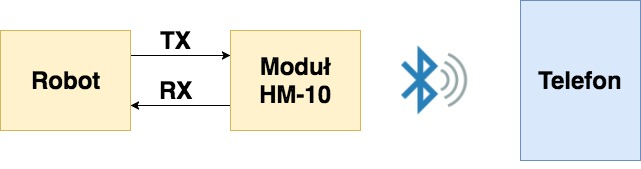
\includegraphics[width=0.75\linewidth]{pic03/bt_communications.jpg}
	\caption{Schemat komunikacji między urządzeniami.}
	\label{fig:communication}	
\end{figure}

Na rysunku ~\ref{fig:communication} przedstawiono schemat komunikacji między robotem a aplikacją mobilną. Aplikacja mobilna komunikuje się radiowo z modułem Bluetooth, który następnie za pomocą przewodów podłączonych do linii TX oraz RX procesora przesyła wysłaną wiadomość.   

\section{Moduł bluetooth}
Z racji, iż docelowym urządzeniem komunikującym się z robotem był telefon iPhone, który obsługuje wyłącznie technologię BLE (ang. \textit{Bluetooth Low Energy}), wybór docelowego modułu komunikacyjnego został mocno ograniczony. Z początku zdecydowano się na moduł Bluetooth HM–11 ze względu na bardzo małe rozmiary. Niestety okazało się, iż owy moduł posiada nietypowy raster, przez co niemożliwym było przylutowanie jakiegokolwiek złącza. Jedynym rozwiązaniem byłoby przylutowanie modułu do płytki elektronicznej robota, aczkolwiek projekt płytki nie przewidywał dodatkowych elementów. W związku z czym zdecydowano się na starszy model HM–10, który dostarczał taką samą funkcjonalność, lecz posiadał gotowe złącze goldpin, które znacząco ułatwiło podłączenie do wyżej wspomnianej płytki. Jedyną wadą zastosowanego modułu był rozmiar.

\begin{figure}[H]
	\centering
		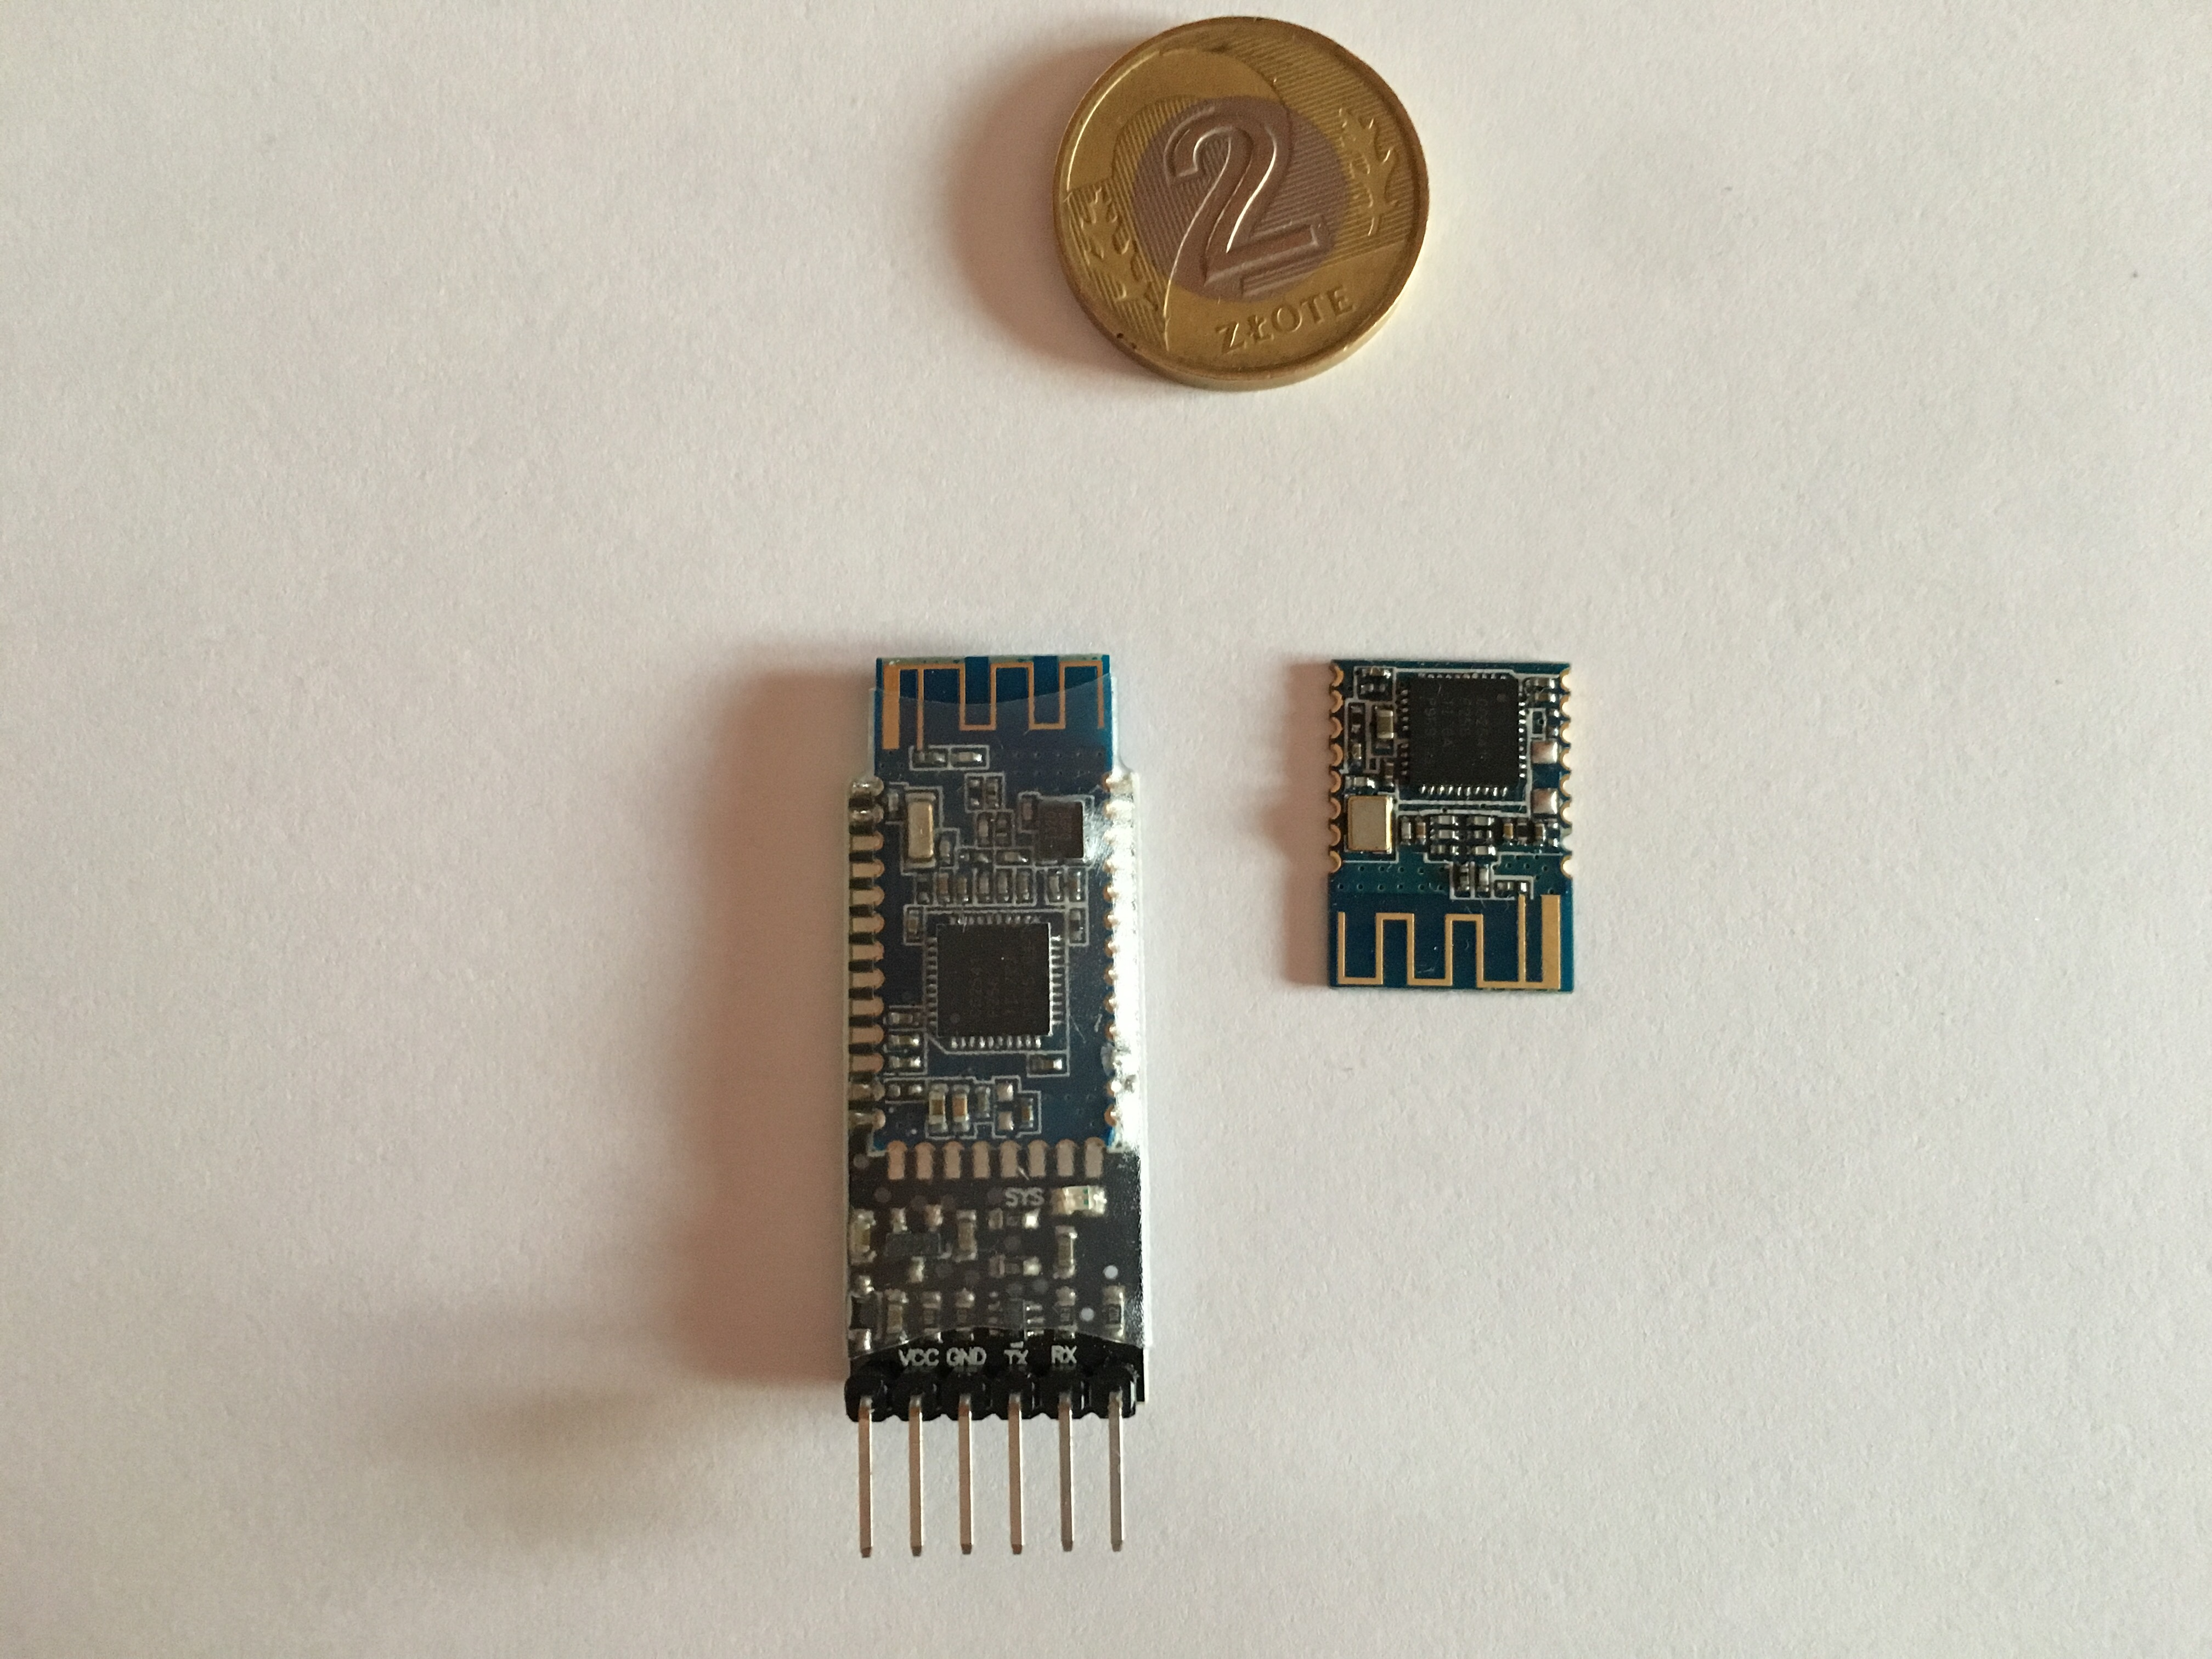
\includegraphics[width=0.75\linewidth]{pic03/bt_modules.jpg}
	\caption{Moduły Bluetooth.}
	\label{fig:bt}	
\end{figure}

Na rysunku ~\ref{fig:bt} po lewej stronie widoczny jest docelowo użyty moduł HM–10, natomiast po prawej wcześniej wspomniany HM–11. U góry ilustracji znajduję się moneta dla odwzorowania rozmiarów omawianych układów.

\section{Realizacja komunikacji}
Komunikacja między urządzeniami bazuje na wysyłaniu ciągu dziesięciu znaków, a dokładniej nieujemnych liczb całkowitych, które następnie są parsowane oraz interpretowane w odpowiedni sposób \cite{Forbot}. Domyślnie wiadomość składa się z dziesięciu zer, a następnie wypełniana jest odpowiednimi wartościami. Poniżej przedstawiono przykładowe formaty wiadomości przesyłane między urządzeniami.

\index{Sensory} \subsubsection{\lstinline$Sensory$}
Komunikacja między urządzeniami rozpoczyna się od wysłania wiadomości przez aplikację mobilną w której pierwsza cyfra wiadomości ma wartość równą 4. Następnie co określony czas robot wysyła wiadomość w której zawarty jest aktualny stan czujników. Komunikacja kończy się w momencie, gdy aplikacja mobilna wyśle wiadomość w której pierwsza cyfra jest różna od 4.

\begin{figure}[H]
	\centering
		
\includegraphics[width=0.75\linewidth]{pic03/sensors.pdf}
	\caption{Schemat wiadomości zawierającej informacje odnośnie stanu sensorów.}
	\label{fig:sensors_communication}	
\end{figure}

Na rysunku ~\ref{fig:sensors_communication} przedstawiono strukturę wiadomości wysłanej przez robota do aplikacji mobilnej. Pierwsza cyfra (równa 4) sygnalizuje aplikacji, iż przesyłana wiadomość zawiera informacje na temat stanu czujników. Cyfry \textit{A, B, C, D} sygnalizują stan cyfrowych czujników wykrywających przeciwnika w sposób binarny (0 – nie wykryto przeciwnika, 1 – wykryto przeciwnika). Cyfry \textit{XX} oraz \textit{YY} informują o stanie analogowych czujników wykrywających koniec ringu (00 – wykryto czarny kolor, 99 – wykryto biały kolor).

\index{Automatyczne sterowanie} \subsubsection{\lstinline$Automatyczne Sterowanie$}

Komunikacja bazuje na jednorazowym wysłaniu wiadomości do robota z poziomu aplikacji mobilnej. Treść wiadomości określa czy robot powinien wstrzymać start do momentu otrzymania komunikatu od sędziego, rodzaj algorytmu walki oraz maksymalną moc silników.

\begin{figure}[H]
	\centering
		
\includegraphics[width=0.75\linewidth]{pic03/automatic.pdf}
	\caption{Schemat wiadomości w której zawarta jest konfiguracja robota.}
	\label{fig:automatic}	
\end{figure}

Rysunek ~\ref{fig:automatic} obrazuje schemat wiadomości wysłanej z aplikacji mobilnej do robota. Pierwsza cyfra (równa 1) informuje, iż robot przechodzi w stan automatycznej jazdy. Cyfra \textit{A} określa numer algorytmu walki (na chwilę obecną występują trzy algorytmy, numerowane 1,2 oraz 3). Kolejna cyfra \textit{B} dostarcza informację odnośnie rodzaju startu (0 – ruch robota rozpoczyna się w~momencie wysłania wiadomości, 1 – robot oczekuje na sygnał sędziego). Ostatnia wartość \textit{XXX} określa procentowo maksymalną moc jaką mogą osiągnąć obydwa silniki (przyjmuje wartości 000 – 100, gdzie 100 oznacza maksymalną moc, a 000 minimalną).

\index{Sterowanie zdalne – akcelerometr} \subsubsection{\lstinline$Sterowanie zdalne - akcelerometr$}

Aplikacja mobilna jednorazowo wysyła komunikat, którego pierwsza cyfra oznacza wejście w~tryb zdalnego sterowania. Następnie wspomniana aplikacja rozpoczyna nasłuchiwanie wiadomości zawierających kierunki ruchu oraz moce poszczególnych silników wysyłanych przez robota.

\begin{figure}[H]
	\centering
		
\includegraphics[width=0.75\linewidth]{pic03/accelerometer.pdf}
	\caption{Schemat wiadomości zdalnego sterowania przy użyciu akcelerometru.}
	\label{fig:accelerometer}	
\end{figure}

Rysunek ~\ref{fig:accelerometer} przedstawia budowę wiadomości wysłanej do aplikacji mobilnej przez robota. Pierwsza cyfra (równa 6) wskazuje, iż robot jest w trybie zdalnego sterowania za pomocą akcelerometru. Kolejne cyfry \textit{A} oraz \textit{B} oznaczają kierunki odpowiedno lewego oraz prawego silnika (1 – obrót w tył, 2 – obrót w przód). \textit{XXX} oraz \textit{YYY} podobnie jak w przypadku trybu automatycznej jazdy określają procentowe moce silników, lewego oraz prawego (przyjmują wartości 000 – 100, gdzie 100 oznacza maksymalną moc, a 000 minimalną).  

